% Created 2020-04-09 Thu 17:49
% Intended LaTeX compiler: pdflatex
\documentclass[11pt]{article}
\usepackage[utf8]{inputenc}
\usepackage[T1]{fontenc}
\usepackage{graphicx}
\usepackage{grffile}
\usepackage{longtable}
\usepackage{wrapfig}
\usepackage{rotating}
\usepackage[normalem]{ulem}
\usepackage{amsmath}
\usepackage{textcomp}
\usepackage{amssymb}
\usepackage{capt-of}
\usepackage{hyperref}
\usepackage[margin=3cm]{geometry}
\author{Alexander Arvidsson}
\date{\today}
\title{Project Log}
\hypersetup{
 pdfauthor={Alexander Arvidsson},
 pdftitle={Project Log},
 pdfkeywords={},
 pdfsubject={},
 pdfcreator={Emacs 26.3 (Org mode 9.4)}, 
 pdflang={English}}
\begin{document}

\maketitle
\tableofcontents

\setlength{\parindent}{0pt}
\setlength{\parskip}{\baselineskip}

\section*{Introduction}
\label{sec:org402d66a}
This page will consist of the collaborative log from each group member and
eventual problems and challenges that the group encounters during the
development process of the project.

Usually, the group will write their own individual efforts at the end of the
week and then compose it into one shared log which will be written here.

\section*{Week 1}
\label{sec:org9b5f427}
This week marks the start of the project, and thus a lot of research and
administrative tasks was required, such as decisions regarding tools and
a schedule.

Every decision that we make during meetings should be documented, so we decided
to create a group contract and a log book. Initially, the log book were only the
individual's own weekly logs, but we later realized we needed a shared log that
summarized the overall progress of the project, which is the log that you are
reading right now.

Here are some decisions that were made during this week:
\begin{itemize}
\item The secretary during the meetings should be rotated according to this order:
\begin{enumerate}
\item Marcus Ansamaa
\item Alexander Arvidsson
\item Anton Håkansson
\item Viktor Truvé
\end{enumerate}
\item The report should be written in  \LaTeX{}
\end{itemize}


We decided to use Google Calendar for scheduled meetings, and that we should
have two lunch meetings as well as 3 workshops every week. The lunch meetings
usually were an hour long, over lunch, while the workshops were all 4 hours,
placed during Thursday afternoon, Friday morning and Friday afternoon.
The purpose of the workshops is to meet up with the group to sit down and get
work done, while also being able to get help from eachother if need be.

For communication, we decided to use Slack as it is the easier
platform which everyone was familiar with, which also gave us a more organized
form of communication than other platforms would offer (for example, Messenger).

File sharing and development ended up being Google Drive and Github. All our
documents and resources we collect during the projects lifetime would be placed
in drive for ease of access, while the project code and report is in two
separate Github repositories for version control.

We got to meet our supervisor during this week which guided us to get a good
start with the project, and we were also able to ask any questions we had before
getting started.

Most of us who were available also attended the introductory seminars during
this week.

The rest of the time was spent invididually, researching different aspects of
the project to get a deeper understanding of what requirements and
specifications our project would need.

\section*{Week 2}
\label{sec:orge6071e4}
This week also had a few lectures, and Alexander also came back from his
vacation so we made sure to get him up to date.

Lots of subjects were brought up during the workshops this week, such as what
method we wanted to use for different parts in the world generator.
We quickly came up with two methods of generating roads, and because we could
not all agree on one method we decided it was best to create two separate demos
that would demonstrate the method and its pros / cons.

The first demo made use of road building Agents that were deployed onto a
2D-plane, and placed down roads while interacting with the road network. This
was initially a very basic system that simply had Agents walk in straight lines
and sometimes branching off into more Agents.

The second demo used a recursive approach where it split the world into small
cells, and each cell could further be subdivided. The idea was to place down a
lot of points, split the cell into two by creating a line between each point,
and then recursively applying that algorithm into more detail.

We decided to postpone selecting which tools to use for our project until next
week, because we wanted to research which tool would suit us best and needed
more time.


In this week we attended a few lectures.
We had our first 3 work meetings, started on the project plan, developed 2 demos
for the road generation, and further discussed the specifications of the
project.
The first road demo made use of road building agents that were deployed onto a
2D-plane, and built outwards.
The second demo used a recursive approach were it split the world into small
cells. We made a lot of admin related decisions. We also researched a bit.

\begin{w-1/2}
\begin{center}
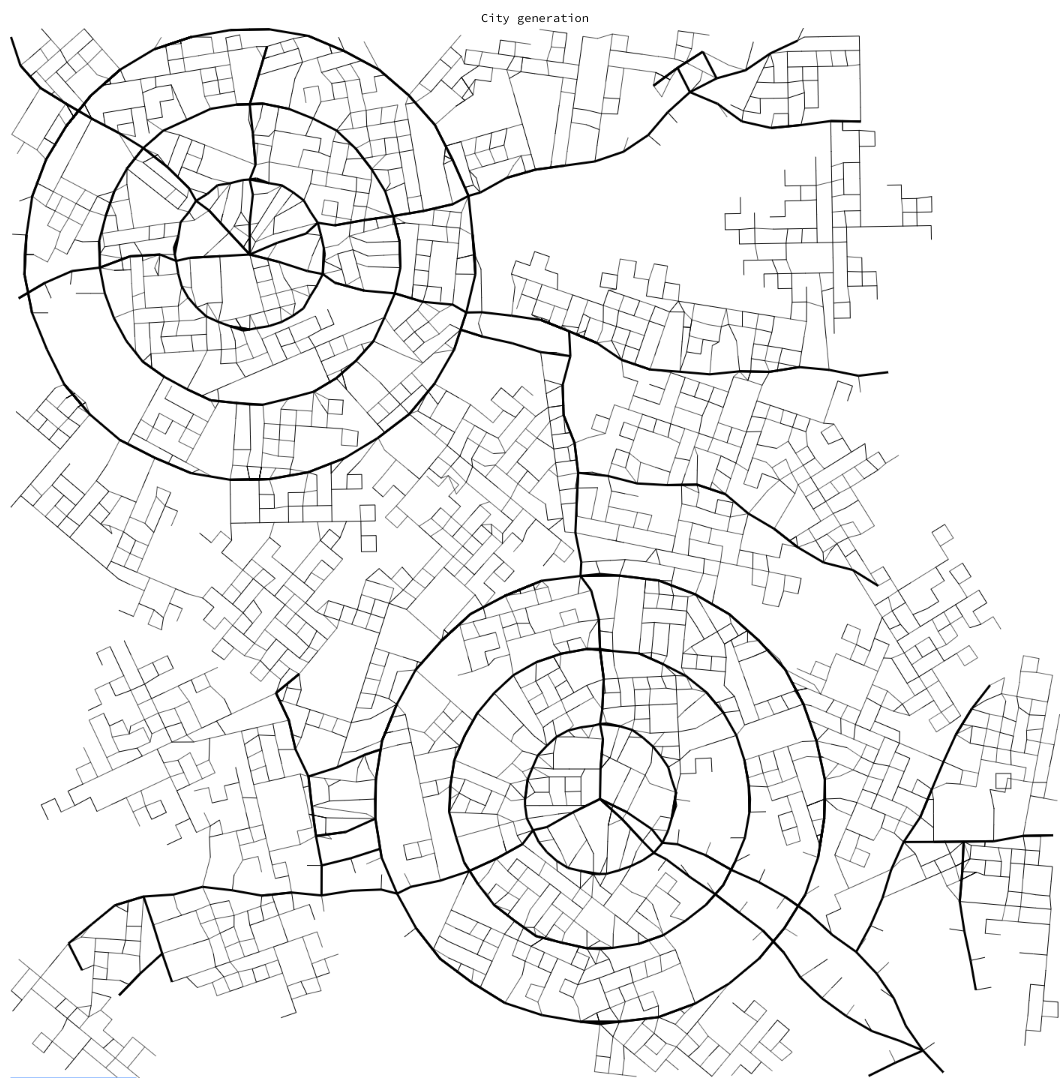
\includegraphics[width=.9\linewidth]{./images/week1/img-000.png}
\end{center}
\end{w-1/2}

\section*{Week 3}
\label{sec:org5481319}
In this week we have put a lot of effort into the project plan. We have finished
a first draft for feedback from the supervisor. We have also decided which tools
(Unity/C\#) we will use to develop the end product.  Furthermore we have also
defined common terminology for referencing the different sections of the road
subdivisioning. We have also expanded the prototypes of road generation with
road strategies for different types of city types (Paris, Washington) and more
natural streets. We have defined a pipeline for the program which essentially
means that we have finalized a design for the algorithm.      

\section*{Week 4}
\label{sec:org8005ad0}
In this week we had a very constructive meeting with Staffan who gave us tips on
how to improve our current project plan. Jacob also set up a Unity-base project.
Although specific sections were originally assigned to be written by project
members eventually all parts of the plan was to some degree rewritten or
modified by someone else. Everyone made an effort to make sure that each of the
chapters were well-written and together made up one coherent text.

\section*{Week 5}
\label{sec:org378b96c}
``In this week we started programming the different generators. Theodor worked with the BuildingGenerator and the PlotGenerator, Viktor worked with the ParkGenerator, Anton and Alexander with the RoadGenerator, Marcus with the TerrainGenerator.
Jacob has worked with FBX export to work in runtime, and had to try a lot of
options to get something to work. One of major problems has been to make the
FbxExporter in Unity to not depend on Editor code. Jacob also made a basic UI
that resembles the mock. Anton worked on generating a road mesh following a
(poly)bezier spline for the Road Generation.''

\section*{Week 6}
\label{sec:orgcbf7955}
In this week everyone kept working on the generators from last week and
improving them. Viktor and Anton also spent time on preparing the half-time
presentation.  The progress in output from the generators will be provided as
images, and more detailed descriptions of how the work progress looked like will
be given in the individual week-logs. Although a very rough draft of it the road
generation logic from Anton and Alexander has started to be merged together. The
park generator is currently in hiatus as Viktor and Theodor work together on
implementing a polygon divider. We have working CI builds and linters now. We
have proper terrain, population, road, park, building (only 1 building type
though). We lack plot and block generator. We also lack a parking generator, but
that wasn't included in the scope of this iteration. Next week we will start a
new iteration. The current FBX exporter only works in editor runtime which is a
major concern.

\section*{Week 7}
\label{sec:orgca7ff6c}
In this week Anton and Viktor held the halftime presentation. Viktor spent most
of the rest of the week after that working on the PathGenerator for the parks,
he was also assisted by Anton. Anton worked on coupling the generated road
network with the spline and road mesh logic(Heavily Assisted by Alexander).
Furthermore, he also has spent some time on generating a more complex shape for
the road mesh (WIP). Jacob wrote on the polygon extractor part of the block
generator. Alex and Jacob merged road generation functionalilty and block gen
inset stuff. Alex implemented the block gen inset stuff. Jacob got a .GLTF and
.GLB exporter to work in runtime. There seems to be some limis to the new
exporter, but it works better than the last one. Marcus worked on adding water
feature to the terrain and tweak the textures.

\section*{Week 8}
\label{sec:orge189878}
This week Anton worked on creating intersections between roads. At the moment
the outline of the intersection looks reasonable - however, no actual complete
mesh is generated except for the arc ``''corners``'' between two roads entering the
intersection.
Alexander has worked on a general noise generator component that can be used in
many parts of the application, and also implemented the noise in the road
generation to create highways outside cities that are guided towards high
populated areas.
Jacob worked on FBX -> glTF for terrain since FBX didn't work without depending
on UnityEditor. Since Unity's terrain is dynamic it doesn't work well in
exporting as model, you can convert it to a mesh but that also requires
UnityEditor. Thus, Jacob worked a lot on converting this terrain into a
mesh-based one, integrating it with noise module, and supporting multiple
textures and such.
Marcus has been working slightly on camera movement so that the user can look
around the city.

\section*{Week 9}
\label{sec:org899bfec}
<Exam week>

\section*{Week 10}
\label{sec:org798326f}
In this week, Marcus has worked on the UI for the terrain generator, adding sea
level, x offset and z offset as modifiable options. A lot of PRs were
reviewed/merged such as Mesh Terrain, Noise module, plots and buildings. We aso
started on the final report and wrote about noise in the Theory chapter. Viktor
spent this week adding the Park Generator to the World Generator and doing a
little bit of report writing. We started doing daily meetings online.
Alexander worked on the road generation so that it now adjusts based on terrain
slopes and sea level in such a way that it doesn't enter seas or tries to ascend
to steep hills. This week Anton spent on reworking the generated road meshes
(simplifying by removing crosssection, only road width and sidewalk now) and
tweaking the intersections to a way that more similarily resembled CityEngine's
intersections(WIP).

\section*{Week 11}
\label{sec:orgc729f88}
Jacob added a skyscraper generator, 5 pages were written on the Theory chapter
(Noise, L-systems, Search-based PCG and Voronoi Diagrams). Marcus has finished
the terrain options: terrain offset and sea level sliders. Using the sliders,
sea level can be adjusted and the user can move along the terrain by entering a
speed given to the sliders.
Alexander worked with improving generation in the UI, like separating the road
and street generation and also implemented block and plot types so that
different things can be generated like parks or skyscrapers.
Anton has also been making improvements on the generated road network mesh. This
includes resolving bugs for specific intersections cases that caused the
intersections and roads to stretch and occupy the whole world. Furthermore, the
same problem was solved for a bug where duplicate identical roads were being
instantiated. The roads also try to project onto the terrain. The projection on
to the terrain is still a work in progress as some segements of the roads appear
underneath the terrain which needs to be resolved next week.
Work has been started with creating what will be the final structure of
BuildingGenerator. The ability of generating any type of building with different
kinds of strategy. Viktor has made sure to get his paths and parks working with
the terrain. He also added a collision-check for the paths and worked on
different algorithms for the paths.``
a




\label{org71dc203}
\bibliographystyle{amsplain}

\label{org92c661b}
\bibliography{references}
\end{document}
